\chapter{Fourier Series}
\begin{enumerate}
	\item The Fourier series of the function $f(x)$ as shown in figure is:
	\begin{figure}[H]
		\centering
		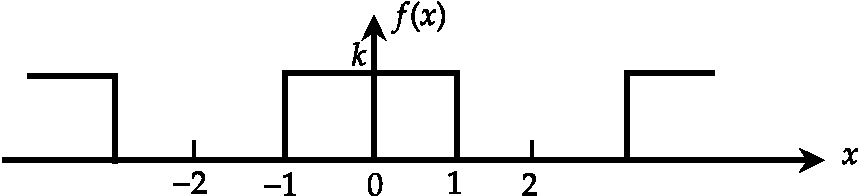
\includegraphics[height=2cm,width=8cm]{FS-assignment-01}
	\end{figure}
	 \begin{tasks}(1)
		\task[\textbf{a.}]$\frac{2 k}{\pi}\left(\cos \frac{\pi}{2} x-\frac{1}{3} \cos \frac{3 \pi}{2} x+\frac{1}{5} \cos \frac{5 \pi}{2} x-+\ldots\right)$
		\task[\textbf{b.}]$\frac{k}{\pi}\left(\cos \frac{\pi}{2} x-\frac{1}{3} \cos \frac{3 \pi}{2} x+\frac{1}{5} \cos \frac{5 \pi}{2} x-+\ldots\right)$
		\task[\textbf{c.}]$\frac{k}{2}+\frac{k}{\pi}\left(\cos \frac{\pi}{2} x-\frac{1}{3} \cos \frac{3 \pi}{2} x+\frac{1}{5} \cos \frac{5 \pi}{2} x-+\ldots\right)$
		\task[\textbf{d.}] $\frac{k}{2}+\frac{2 k}{\pi}\left(\cos \frac{\pi}{2} x-\frac{1}{3} \cos \frac{3 \pi}{2} x+\frac{1}{5} \cos \frac{5 \pi}{2} x-+\ldots\right)$
	\end{tasks}
\begin{answer}
	\begin{align*}
	f(x)&=\left\{\begin{array}{clc}0 & \text { if } & -2<x<-1 \\ k & \text { if } & -1<x<1 \\ 0 & \text { if } & 1<x<2\end{array} \quad p=2 L=4, L=2\right.\\
	\text{Let }f(x)&=a_{0}+\sum_{n=1}^{\infty}\left(a_{n} \cos \frac{n \pi}{L} x+b_{n} \sin \frac{n \pi}{L} x\right)\\
	\because a_{0}&=\frac{1}{2 L} \int_{-L}^{L} f(x) d x\\
	\Rightarrow a_{0}&=\frac{1}{4} \int_{-2}^{2} f(x) d x=\frac{1}{4} \int_{-1}^{1} k d x=\frac{k}{2}\\
	\because a_{n}&=\frac{1}{L} \int_{-L}^{L} f(x) \cos \frac{n \pi x}{L} d x\\
	\Rightarrow a_{n}&=\frac{1}{2} \int_{-2}^{2} f(x) \cos \frac{n \pi x}{2} d x=\frac{1}{2} \int_{-1}^{1} k \cos \frac{n \pi x}{2} d x\\
	\Rightarrow a_{n}&=\frac{k}{2}\left[\frac{2}{n \pi} \sin \frac{n \pi x}{2}\right]_{-1}^{1}=\frac{2 k}{n \pi} \sin \frac{n \pi}{2}=\left\{\begin{array}{cl}0, & n=2,4,6 \ldots . \\ \frac{2 k}{n \pi}, & n=1,5,9 \ldots . . \\ -\frac{2 k}{n \pi}, & n=3,7,11 \ldots . .\end{array}\right.\\
	\because b_{n}&=\frac{1}{L} \int_{-L}^{l} f(x) \sin \frac{n \pi x}{L} d x\\
	\Rightarrow b_{n}&=\frac{1}{2} \int_{-2}^{2} f(x) \sin \frac{n \pi x}{2} d x=\frac{1}{2} \int_{-1}^{1} k \sin \frac{n \pi x}{2} d x=\frac{k}{2}\left[-\frac{2}{n \pi} \cos \frac{n \pi x}{2}\right]_{-1}^{1}=0\\
	\text{Thus Fourier series is }f(x)&=\frac{k}{2}+\frac{2 k}{\pi}\left(\cos \frac{\pi}{2} x-\frac{1}{3} \cos \frac{3 \pi}{2} x+\frac{1}{5} \cos \frac{5 \pi}{2} x-+\ldots\right)
	\end{align*}
	So the correct option is \textbf{Option (d)}
\end{answer}
	\item The Fourier series of the periodic function
	$$
	f(x)=e^{x} ; \quad(-\pi<x<\pi), \quad \text { having period } 2 \pi \text { is }
	$$
	 \begin{tasks}(1)
		\task[\textbf{a.}]$\frac{1}{\pi}\left[\frac{1}{2}-\frac{1}{1^{2}}(\cos x-\sin x)+\frac{1}{2^{2}}(\cos 2 x-2 \sin 2 x)-+\ldots\right]$
		\task[\textbf{b.}]$\frac{2}{\pi}\left[\frac{1}{2}-\frac{1}{1^{2}}(\cos x-\sin x)+\frac{1}{2^{2}}(\cos 2 x-2 \sin 2 x)-+\ldots\right]$
		\task[\textbf{c.}] $\frac{\sinh \pi}{\pi}\left[\frac{1}{2}-\frac{1}{1+1^{2}} \cdot(\cos x-\sin x)+\frac{1}{1+2^{2}}(\cos 2 x-2 \sin 2 x)-+\ldots\right]$
		\task[\textbf{d.}] $\frac{2 \sinh \pi}{\pi}\left[\frac{1}{2}-\frac{1}{1+1^{2}}(\cos x-\sin x)+\frac{1}{1+2^{2}}(\cos 2 x-2 \sin 2 x)-+\ldots\right]$
	\end{tasks}
\begin{answer}
	\begin{align*}
&\text{	Let Fourier series is }f(x)=\sum_{n=\infty}^{\infty} c_{n} e^{i n x}\\
\because c_{n}&=\frac{1}{2 \pi} \int_{-\pi}^{\pi} f(x) e^{-i n x} d x\\
\Rightarrow c_{n}&=\frac{1}{2 \pi} \int_{-\pi}^{\pi} e^{x} e^{-i n x} d x=\frac{1}{2 \pi} \int_{-\pi}^{\pi} e^{(1-i n) x} d x=\frac{1}{2 \pi} \frac{1}{(1-i n)}\left[e^{(1-i n) x}\right]_{-\pi}^{\pi}=\frac{1}{2 \pi} \frac{1}{(1-i n)}\left[e^{(1-i n) \pi}-e^{-(1-i n) \pi}\right]\\
\Rightarrow c_{n}&=\frac{1}{2 \pi} \frac{1}{(1-i n)}\left[e^{\pi} e^{-i n \pi}-e^{-\pi} e^{i n \pi}\right]=\frac{1}{2 \pi}\left(\frac{1+i n}{1+n^{2}}\right)\left[e^{\pi}-e^{-\pi}\right](-1)^{n} \quad \because e^{\pm i n \pi}=(-1)^{n}\\
\Rightarrow c_{n}&=\left(\frac{1+i n}{1+n^{2}}\right) \frac{\sinh \pi}{\pi}(-1)^{n} \quad \quad \because \sinh \pi=\frac{e^{\pi}-e^{-\pi}}{2}
	\end{align*}
	\begin{align}
	\text{Thus Fourier series is }f(x)&=\frac{\sinh \pi}{\pi} \sum_{n=-\infty}^{\infty}(-1)^{n}\left(\frac{1+i n}{1+n^{2}}\right) e^{i n x}\label{FS-01}
	\intertext{Let us derive the real Fourier series}\notag
	\because(1+i n) e^{i n x}&=(1+i n)(\cos n x+i \sin n x)=(\cos n x-n \sin n x)+i(\cos n x+\sin n x)\notag\\
	\because n\text{ varies from }&\text{ $-\infty$ to $+\infty$, equation (\ref{FS-01}) has corresponding term with $-n$ instead of $n$.}\notag
	\intertext{Thus}
	f(x)&=\frac{\sinh \pi}{\pi}+2 \frac{\sinh \pi}{\pi} \sum_{n=1}^{\infty}(-1)^{n} \frac{(\cos n x-n \sin n x)}{1+n^{2}}\notag\\
	f(x)&=\frac{2 \sinh \pi}{\pi}\left[\frac{1}{2}-\frac{1}{1+1^{2}}(\cos x-\sin x)+\frac{1}{1+2^{2}}(\cos 2 x-2 \sin 2 x)-+\ldots\right]\notag
	\end{align}
		So the correct option is \textbf{Option (d)}
\end{answer}
	\item  A sinusoidal voltage $E_{0} \sin \omega t$ where $t$ is time is passed through half-wave rectifier that clips the negative portion of the wave.
$f(t)=\left\{\begin{array}{ccc}0 & \text { if } & -\frac{\pi}{\omega}<t<0 \\ E_{0} \sin \omega t & \text { if } & 0<t<\frac{\pi}{\omega}\end{array}\right.$
	Then the Fourier series of the resulting periodic function is
	\begin{figure}[H]
		\centering
		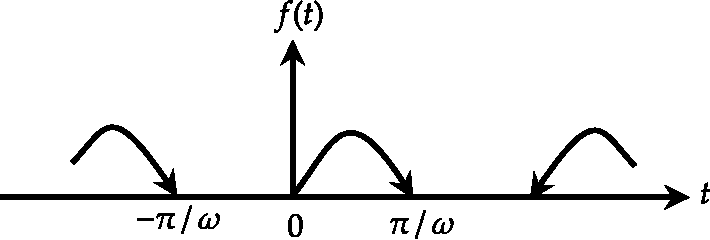
\includegraphics[height=2.5cm,width=8cm]{FS-assignment-02}
	\end{figure}
	 \begin{tasks}(1)
		\task[\textbf{a.}]$f(t)=a_{0}+b_{1} \sin \omega t+\sum_{n=2.4}^{\infty} \frac{2 E_{0}}{\pi\left(1-n^{2}\right)} \cos n \omega t$
		\task[\textbf{b.}] $f(t)=a_{0}+b_{1} \sin \omega t+\sum_{n=1,2,3_{1}, .}^{\infty} \frac{2 E_{0}}{\pi\left(1-n^{2}\right)} \cos n \omega t$
		\task[\textbf{c.}]$f(t)=b_{1} \sin \omega t+\sum_{n=2,4 \ldots}^{\infty} \frac{2 E_{0}}{\pi\left(1-n^{2}\right)} \cos n \omega t$
		\task[\textbf{d.}] $f(t)=\sum_{n=2,4 \ldots}^{\infty} \frac{2 E_{0}}{\pi\left(1-n^{2}\right)} \cos n \omega t$
	\end{tasks}
\begin{answer}
	\begin{align*}
	f(t)&=\left\{\begin{array}{cl}0 & \text { if } \quad-\frac{\pi}{\omega}<t<0 \\ E_{0} \sin \omega t & \text { if } \quad 0<t<\frac{\pi}{\omega}\end{array} \quad p=2 L=2 \frac{\pi}{\omega}, L=\frac{\pi}{\omega}\right.\\
	\text{Let }f(x)&=a_{0}+\sum_{n=1}^{\infty}\left(a_{n} \cos \frac{n \pi}{L} x+b_{n} \sin \frac{n \pi}{L} x\right)\\
	\because a_{0}&=\frac{1}{2 L} \int_{-L}^{L} f(t) d t \Rightarrow a_{0}=\frac{\omega}{2 \pi} \int_{-\pi / \omega}^{\pi / \omega} f(t) d t=\frac{\omega}{2 \pi} \int_{0}^{\pi / \omega} E_{0} \sin \omega t d t\\
	\Rightarrow a_{0}&=\frac{\omega}{2 \pi}\left[-\frac{E_{0}}{\omega} \cos \omega t\right]_{0}^{\pi / \omega}=\frac{E_{0}}{\pi}\\
	\because a_{n}&=\frac{1}{L} \int_{-L}^{L} f(t) \cos \frac{n \pi t}{L} d t\\
	\Rightarrow a_{n}&=\frac{\omega}{\pi} \int_{-\pi / \omega}^{\pi / \omega} f(t) \cos n \omega t d t=\frac{\omega}{\pi} \int_{0}^{\pi / \omega} E_{0} \sin \omega t \cos n \omega t d t=\frac{E_{0} \omega}{2 \pi} \int_{0}^{\pi / \omega} 2 \sin \omega t \cos n \omega t d t\\
	\Rightarrow a_{n}&=\frac{E_{0} \omega}{2 \pi} \int_{0}^{\pi / \omega}[\sin (1+n) \omega t+\sin (1-n) \omega t] d t\\
	\text { For } n&=1 ; \quad a_{1}=\frac{E_{0} \omega}{2 \pi} \int_{0}^{\pi / \omega} \sin 2 \omega t d t=\frac{E_{0} \omega}{2 \pi}\left[\frac{-\cos 2 \omega t}{2 \omega}\right]_{0}^{\pi / \omega}=0\\
	\text{For }n&=2,3,4 \ldots\\
	\Rightarrow a_{n}&=\frac{E_{0} \omega}{2 \pi}\left[-\frac{\cos (1+n) \omega t}{(1+n) \omega}-\frac{\cos (1-n) \omega t}{(1-n) \omega}\right]_{0}^{\pi / \omega}\\
	\Rightarrow a_{n}&=\frac{E_{0}}{2 \pi}\left[\frac{-\cos (1+n) \pi+1}{(1+n)}+\frac{-\cos (1-n) \pi+1}{(1-n)}\right]=\left\{\begin{array}{cc}0 & n=3,5,7 \ldots \\ \frac{2 E_{0}}{\pi\left(d-n^{2}\right)} & n=2,4,6 \ldots\end{array}\right.\\
	\because b_{n}&=\frac{1}{L} \int_{-L}^{L} f(x) \sin \frac{n \pi x}{L} d x\\
	\Rightarrow b_{n}&=\frac{\omega}{\pi} \int_{-\pi / \omega}^{\pi / \omega} f(t) \sin n \omega t d t=\frac{\omega}{\pi} \int_{0}^{\pi / \omega} E_{0} \sin \omega t \sin n \omega t d t=\frac{E_{0} \omega}{2 \pi} \int_{0}^{\pi / \omega} 2 \sin \omega t \sin n \omega t d t\\
	\Rightarrow b_{n}&=\frac{E_{0} \omega}{2 \pi} \int_{0}^{\pi / \omega}[-\cos (1+n) \omega t+\cos (1-n) \omega t] d t\\
	\text{For }n&=1\\
	b_{1}&=\frac{E_{0} \omega}{2 \pi} \int_{0}^{\pi / \omega}[1-\cos 2 \omega t] d t=\frac{E_{0} \omega}{2 \pi} \int_{0}^{\pi / \omega}\left[t-\frac{\sin 2 \omega t}{2 \omega}\right]_{0}^{\pi / \omega}=\frac{E_{0} \omega}{2 \pi} \frac{\pi}{\omega}=\frac{E_{0}}{2}\\
	\text{For }n&=2,3,4 \ldots .\\
	\Rightarrow b_{n}&=\frac{E_{0} \omega}{2 \pi}\left[-\frac{\sin (1+n) \omega t}{(1+n) \omega}+\frac{\sin (1-n) \omega t}{(1-n) \omega}\right]_{0}^{\pi / \omega}=\frac{E_{0}}{2 \pi}\left[\frac{-\sin (1+n) \pi}{(1+n)}+\frac{\sin (1-n) \pi}{(1-n)}\right]=0
	\intertext{Thus Fourier series}
	f(t)&=a_{0}+b_{1} \sin \omega t+\sum_{n=2,4}^{\infty} a_{n} \cos n \omega t=a_{0}+b_{1} \sin \omega t+\sum_{n=2,4 \ldots}^{\infty} \frac{2 E_{0}}{\pi\left(1-n^{2}\right)} \cos n \omega t
	\end{align*}
		So the correct option is \textbf{Option (a)}
\end{answer}
	\item  The Fourier series of even periodic expansion of the function $f(x)$ as shown in figure below is
	\begin{figure}[H]
		\centering
		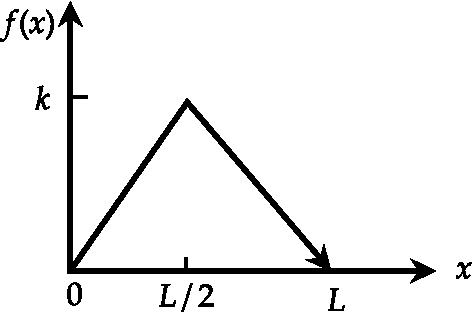
\includegraphics[height=3cm,width=5cm]{FS-assignment-03}
	\end{figure}
	$f(x)=\left\{\begin{array}{clc}\frac{2 k}{L} x & \text { if } & 0<x<\frac{L}{2} \\ \frac{2 k}{L}(L-x) & \text { if } & \frac{L}{2}<x<L\end{array}\right.$
	 \begin{tasks}(1)
		\task[\textbf{a.}]$f(x)=\frac{4 k}{\pi^{2}}\left(\frac{1}{2^{2}} \cos \frac{2 \pi x}{L}+\frac{1}{6^{2}} \cos \frac{6 \pi x}{L}+\frac{1}{10^{2}} \cos \frac{10 \pi x}{L}+\ldots \ldots\right)$
		\task[\textbf{b.}]$f(x)=\frac{k}{2}-\frac{4 k}{\pi^{2}}\left(\frac{1}{2^{2}} \cos \frac{2 \pi x}{L}+\frac{1}{6^{2}} \cos \frac{6 \pi x}{L}+\frac{1}{10^{2}} \cos \frac{10 \pi x}{L}+\ldots .\right)$
		\task[\textbf{c.}]$f(x)=\frac{k}{2}-\frac{16 k}{\pi^{2}}\left(\frac{1}{2^{2}} \sin \frac{2 \pi x}{L}+\frac{1}{6^{2}} \sin \frac{6 \pi x}{L}+\frac{1}{10^{2}} \sin \frac{10 \pi x}{L}+\ldots . .\right)$
		\task[\textbf{d.}] $f(x)=\frac{k}{2}-\frac{16 k}{\pi^{2}}\left(\frac{1}{2^{2}} \cos \frac{2 \pi x}{L}+\frac{1}{6^{2}} \cos \frac{6 \pi x}{L}+\frac{1}{10^{2}} \cos \frac{10 \pi x}{L}+\ldots .\right)$
	\end{tasks}
\begin{answer}
	Even periodic extension
	\begin{figure}[H]
		\centering
		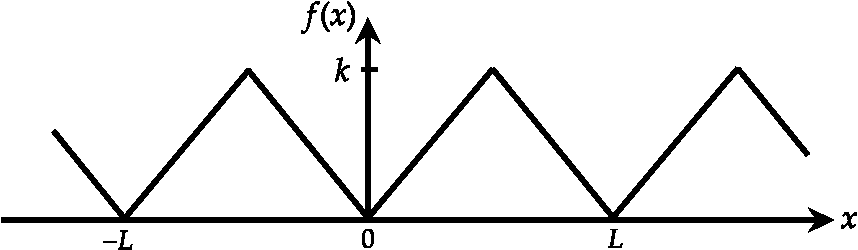
\includegraphics[height=2.5cm,width=8cm]{FS-assignment-04}
	\end{figure}
	\begin{align*}
	\because a_{0}&=\frac{1}{L} \int_{0}^{L} f(x) d x\\
	\Rightarrow a_{0}&=\frac{1}{L}\left[\frac{2 k}{L} \int_{0}^{\frac{L}{2}} x d x+\frac{2 k}{L} \int_{\frac{L}{2}}^{L}(L-x) d x\right]=\frac{k}{2}\\
	\because a_{n}&=\frac{2}{L} \int_{0}^{L} f(x) \cos \frac{n \pi x}{L} d x\\
	\Rightarrow a_{n}&=\frac{1}{L}\left[\frac{2 k}{L} \int_{0}^{\frac{L}{2}} x \cos \frac{n \pi x}{L} d x+\frac{2 k}{L} \int_{\frac{L}{2}}^{L}(L-x) \cos \frac{n \pi x}{L} d x\right]
	\intertext{Let us calculate the integral}
	\int_{0}^{\frac{L}{2}} x \cos \frac{n \pi x}{L} d x&=\frac{L}{n \pi}\left[x \sin \frac{n \pi x}{L}\right]_{0}^{L / 2}+\left(\frac{L}{n \pi}\right)^{2}\left[\cos \frac{n \pi x}{L}\right]_{0}^{L / 2}\\
	\Rightarrow \int_{0}^{\frac{L}{2}} x \cos \frac{n \pi x}{L} d x&=\frac{L^{2}}{2 n \pi} \sin \frac{n \pi}{2}+\frac{L^{2}}{n^{2} \pi^{2}}\left(\cos \frac{n \pi}{2}-1\right)\\
	\text{and }\int_{L / 2}^{L}(L-x) \cos \frac{n \pi x}{L} d x&=\frac{L}{n \pi}\left[(L-x) \sin \frac{n \pi x}{L}\right]_{L / 2}^{L}-\left(\frac{L}{n \pi}\right)^{2}\left[\cos \frac{n \pi x}{L}\right]_{L / 2}^{L}\\
	\Rightarrow \int_{L / 2}^{L}(L-x) \cos \frac{n \pi x}{L} d x&=-\frac{L^{2}}{2 n \pi} \sin \frac{n \pi}{2}-\frac{L^{2}}{n^{2} \pi^{2}}\left(\cos n \pi-\cos \frac{n \pi}{2}\right)\\
	\Rightarrow a_{n}&=\frac{1}{L}\left[\frac{2 k}{L} \int_{0}^{\frac{L}{2}} x \cos \frac{n \pi x}{L} d x+\frac{2 k}{L} \int_{\frac{L}{2}}^{L}(L-x) \cos \frac{n \pi x}{L} d x\right]=\frac{4 k}{n^{2} \pi^{2}}\left(2 \cos \frac{n \pi}{2}-\cos n \pi-1\right)\\
	\Rightarrow a_{2}&=-\frac{16 k}{2^{2} \pi^{2}}, a_{6}=-\frac{16 k}{6^{2} \pi^{2}}, a_{10}=-\frac{16 k}{10^{2} \pi^{2}}, \ldots \ldots \ldots . . \text{and }a_{n}=0\text{ if }n \neq 2,6,10 \ldots .
	\intertext{Hence the first half-range expansion of $f(x)$ is}                  
	f(x)&=\frac{k}{2}-\frac{16 k}{\pi^{2}}\left(\frac{1}{2^{2}} \cos \frac{2 \pi x}{L}+\frac{1}{6^{2}} \cos \frac{6 \pi x}{L}+\frac{1}{10^{2}} \cos \frac{10 \pi x}{L}+\ldots . .\right)  
	\intertext{This Fourier cosine series represents the even periodic extension of the given function $f(x)$, of period $2 L$ as shown in figure.}     
	\end{align*}
	So the correct option is \textbf{Option (d)}
\end{answer}
\item  The total square error of $F$ with $N=3$ relative to
$$
f(x)=x+\pi \quad(-\pi<x<\pi)
$$
on the interval $-\pi \leq x \leq \pi$ is
	 \begin{tasks}(2)
		\task[\textbf{a.}]$E^{*}=\frac{8}{3} \pi^{3}-\pi\left[2 \pi^{2}+\frac{49}{9}\right]$
		\task[\textbf{b.}]$E^{*}=\frac{4}{3} \pi^{3}-\pi\left[2 \pi^{2}+\frac{49}{9}\right]$
		\task[\textbf{c.}]$E^{*}=\frac{8}{3} \pi^{3}-\pi\left[\pi^{2}+\frac{49}{9}\right]$
		\task[\textbf{d.}] $E^{*}=\frac{8}{3} \pi^{3}-\left[2 \pi^{2}+\frac{49}{9}\right]$
	\end{tasks}
	\begin{answer}
		\begin{align*}
		\text{Fourier coefficients are }a_{0}&=\pi, a_{n}=0\text{ and } b_{n}=-\frac{2}{n} \cos n \pi.\\
		\text{Its Fourier series is given by }F(x)&=\pi+2 \sin x-\sin 2 x+\frac{2}{3} \sin 3 x.
		\intertext{Hence}
		E^{*}=\int_{-\pi}^{\pi} f^{2} d x-\pi\left[2 a_{0}^{2}+\sum_{n=1}^{N}\left(a_{n}^{2}+b_{n}^{2}\right)\right]&=\int_{-\pi}^{\pi}(x+\pi)^{2} d \dot{x}-\pi\left[2 \pi^{2}+2^{2}+1^{2}+\left(\frac{2}{3}\right)^{2}\right]\\
		E^{*}&=\frac{8}{3} \pi^{3}-\pi\left[2 \pi^{2}+\frac{49}{9}\right]
		\end{align*}
		So the correct option is \textbf{Option (a)}	
	\end{answer}
	
	
	
	
	
\end{enumerate}